\chapter{Time Series Clustering}

This chapter first gives a definition of a time series that will be used throughout the paper, it goes on to give an overview of the different time series clustering approaches and finally discusses the different representation methods, and clustering algorithms encountered in the literature. 

\subsubsection*{What is a time series}
In this report we will deal with \textit{discrete time series}. 
A time series is defined as a set of observations $\{x_t\}$ recorded at a specific time $t$. 
A discrete time series is a time series where the set of times when observations are made ($T_0$) is discrete \cite{brockwell_davis_advanced}. 
A multivariate time series can be viewed as a set of vectors $\{\mathbf{x}_t\}$ where each set of vector elements $\{x^i_t\}$ is an individual time series. 
This means that the elements of the same vector $[x^1_t, x^2_t,...,x^N_t]$ are separate observations made at the same time instance $t$. 
In a wind turbine, measurements of the temperature in the gear box made every 10 seconds can be considered a univariate time series. 
While the set of measurements made every 10 seconds of the temperature in the gear box, the power produced by the turbine, and the wind speed ahead of the blades can be considered a multivariate time series. \bigskip

\section{Overview of Time Series Clustering}
There are three types of TSC, \textit{whole-series TSC}, \textit{subsequence TSC} and \textit{time-point TSC}. 
Whole-series TSC is when multiple ''whole'' time series are clustered with respect to each other. 
Subsequence TSC comprises the clustering of subsequences of the same time series with respect to each other. 
The defining difference between whole-series and subsequence TSC is that whole-series TSC clusters multiple time series while subsequence TSC clusters clusters different subsequences of the same time series. 
When performing time-point TSC the goal is to cluster individual observations of a time series wrt. to each other. 
In this review we will only consider work using whole-series TSC, so when the phrase \textit{time-series clustering} is used, one can assume that whole-series TSC is what is being refered to. \bigskip

Whole series TSC can broadly be divided into three main approaches. 
The raw-data based approach, the feature-based approach and the model based approach. 
In the raw-data based approach one measures the similarity between the raw time series themselves and clusters them based on this. 
When clustering raw time series the majority of the work goes into selection of similarity metric and clustering algorithm, and one clusters the time series with regard to similarity in time or similarity in shape \cite{tsc_rev}. 
In the feature-based approach one also clusters time series with regard to similarity in time, and shape, but the work is somewhat shifted away from choice of similarity metric and over to choice of representation. 
Either to extract more relevant information from the time series, or to reduce the computational complexity of the similarity measurement. 
In the model-based approach the goal most often to cluster time series with regard to the underlying data generating process \cite{moar_mpl_tsc}.
The underlying assumption being that two time series that appear different might still have been generated by the same process.

\begin{figure}
    \begin{center}
    \tikzstyle{int} = [pin edge={to-,thin,black}]
\tikzstyle{sqr}  = [rectangle, rounded corners, minimum width=4.25cm, minimum height=1cm,text centered, draw=black, fill=white]
\tikzstyle{arrow} = [thin,->,>=stealth]

\begin{tikzpicture}[node distance=1.75cm]

%% Model-based approach
\node (inp_mod) [int] {Raw time series};
\node (rep_mod) [sqr, below of=inp_mod] {Model parameters};
\node (sim_mod) [sqr, below of=rep_mod] {Similarity measurement};
\node (clu_mod) [sqr, below of=sim_mod] {Clustering};
\node (out_mod) [int, below of=clu_mod] {Clusters};

%% Feature-based approach
\node (inp_fea) [int, right of=inp_mod, xshift=3cm] {Raw time series};
\node (rep_fea) [sqr, below of=inp_fea] {Extracted features};
\node (sim_fea) [sqr, below of=rep_fea] {Similarity measurement};
\node (clu_fea) [sqr, below of=sim_fea] {Clustering};
\node (out_fea) [int, below of=clu_fea] {Clusters};

%% Raw-data based approach
\node (inp_raw) [int, right of=inp_fea, xshift=3cm] {Raw time series};
\node (sim_raw) [sqr, right of=sim_fea, xshift=3cm] {Similarity measurement};
\node (clu_raw) [sqr, below of=sim_raw] {Clustering};
\node (out_raw) [int, below of=clu_raw] {Clusters};

%% Names
\node (nam_mod) [int, below of=out_mod, yshift=1cm] {\textbf{(Model-based)}};
\node (nam_fea) [int, below of=out_fea, yshift=1cm] {\textbf{(Feature-based)}};
\node (nam_raw) [int, below of=out_raw, yshift=1cm] {\textbf{(Raw-data based)}};

%% Arrows
\draw [arrow] (inp_mod) -- (rep_mod);
\draw [arrow] (rep_mod) -- (sim_mod);
\draw [arrow] (sim_mod) -- (clu_mod);
\draw [arrow] (clu_mod) -- (out_mod);

\draw [arrow] (inp_fea) -- (rep_fea);
\draw [arrow] (rep_fea) -- (sim_fea);
\draw [arrow] (sim_fea) -- (clu_fea);
\draw [arrow] (clu_fea) -- (out_fea);

\draw [arrow] (inp_raw) -- (sim_raw);
\draw [arrow] (sim_raw) -- (clu_raw);
\draw [arrow] (clu_raw) -- (out_raw);
\end{tikzpicture}
    \end{center}
    \caption{Illustration of the three approaches to TSC, and their components. The illustration is inspired by figure 2 in \textcite{tsc_rev}}.
    \label{fig:tsc_approaches}
\end{figure}

The common denominator of the three approaches to TSC mentioned is that they are all made up of three distinct parts: representation method, similarity metric and clustering algorithm. 
This is illustrated in figure \ref{fig:tsc_approaches}.
The choice of representation is key, and is the task of retaining the valuable information while disregarding the irrelevant information. 
When calculating the similarity between all combinations of time series one is clustering, the resulting similarity measures are stored in what is called a \textit{dissimilarity matrix}.
The choice of similarity metric is important in a raw-data approach as it decides which aspects of the time series will be used to measure (dis)similarity, and has a has a significant impact on the time-complexity of the clustering system. 
However the requirements of similarity measure are somewhat relaxed in the feature-based and model-based approaches as the representation method already limits the number of aspects which one can compare time series with, so many of the same similarity measures are used.

\section{Time Series Models and Representations} \label{sec:ts_models}
To select suitable mathematical models for a dataset, we have to allow for the random nature of future observations. 
This is done by assuming that each observation in a time series $x_t$ is a realization of a particular random variable $X_t$. 
The time series can then be modelled as a collection/set of random variables $\{X_t\}$, also known as a \textit{stochastic process} \cite{brockwell_davis_advanced}. 
In the following subsections the theory of the three most prevalant will be presented: ARMA models, HMM and PCA.

\subsection{Autoregressive Moving Average Model}
To define an ARMA model, one needs to have a clear understanding of the terms white noise process, and stationary process. 
We say that the stochastic process $\{Z_t\}$ is ''white noise'' with zero mean, and variance $\sigma^2$ ($\{Z_t\} \sim WN(0, \sigma^2)$) if and only if $\{Z_t\}$ is zero mean, and every random variable contained in $\{Z_t\}$ is uncorrelated with every other random variable contained in $\{Z_t\}$. 
A stochastic process $\{X_t\}$ is said to be weakly wide-sense stationary if the mean, and variance are constant for all terms in the process. 
$\{X_t\}$ is said to be weakly short-term stationary if the mean and variance of terms are constant for distinct time periods within the duration of the process, but are not constant for all terms in the process. 
For brevity the term ''stationary process'' will be used when refering to a \textit{weakly wide-sense stationary process}. 
An ARMA model descirbes a time series in terms of difference equations. 
It can be considered a combination of two smaller models, an autoregressive (AR) model and a moving average (MA) model. 
Let $\{X_t\}$ be a stationary process. 
An $\mathrm{MA}(q)$ model will describe every term $X_t$ as a linear combination of $q$ distinct white noise terms as in equation \eqref{eq:MA_q}.

\begin{equation}
    X_t = Z_{t} + \theta_1 Z_{t-1} + ... + \theta_q Z_{t-q}
    \label{eq:MA_q}
\end{equation}

Whereas an $\mathrm{AR}(p)$ model will describe every term $X_t$ as a linear combination of $p$ previous terms of $\{X_t\}$ as in equation \eqref{eq:AR_p}

\begin{equation}
    X_t = \phi_1 X_{t-1} + ... + \phi_p X_{t-p}
    \label{eq:AR_p}
\end{equation}

Putting equations \eqref{eq:AR_p} and \eqref{eq:MA_q} together, an $\mathrm{ARMA}(p,q)$ model will describe every term $X_t$ as a linear combination of $p$ previous terms, and $q$ white noise terms as in equation \eqref{eq:ARMA_p_q}.

\begin{equation}
    X_t - \phi_1 X_{t-1} - ... - \phi_p X_{t-p} = Z_{t} + \theta_1 Z_{t-1} + ... + \theta_q Z_{t-q}
    \label{eq:ARMA_p_q}
\end{equation}

Given that the polynomials $1 + \theta_1 z + \theta_2 z^2 + ... + \theta_q z^q$ and $1 - \phi_1 z - \phi_2 z^2 - ... - \phi_p z^p$ have no common factors \cite{brockwell_davis}.
When modelling a time series with an ARMA model, one usually attempts to decompose the time series into a set of components, as shown in equation \eqref{eq:ts_comp}. 
Here $X_t$ is the observed time series, 
$r_t$ is called the trend component, 
$s_t$ is called the seasonal component, 
$c_t$ is called the cyclical component 
and $\epsilon_t$ is called the innovations or residual component. 

\begin{equation}
    X_t = r_t + s_t + c_t + \epsilon_t
    \label{eq:ts_comp}
\end{equation}

$r_t$, $s_t$ and $c_t$ represent the deterministic components of trend, shirt term periodic behaviour and long term periodic behaviour components of the time series respectively. 
$\epsilon_t$ represent the random component of the time series, and is often the component of the time series one attempts to model with an ARMA model. 

\subsection{Hidden Markov Models} \label{s:hmm}
Let $\{X_n\}$ be a stochastic process where the random variables contained in $\{X_n\}$ only can take on a finite number of values which we will call states. 
Let $X_n$ denote the state at time period $n$. 
The probability of $X_n$ transitioning from state $i$ to state $j$ at the next time period $n+1$ is called the transition probability, and is denoted $p_{ij}$. 
It seems natural that $p_{ij}$ is conditional on what the state has been in previous time periods. 
$\{X_t\}$ is said to be a \textit{Markov chain} if $p_{ij}$ only is conditional on the past state, as shown in equation \eqref{eq:markov_property}.

\begin{equation}
    \begin{split}
        p_{ij}  &= P(X_n = i | X_{n-1} = i_{n-1}, X_{n-2} = i_{n-2},..., X_{1} = i_{1}, X_{0} = i_{0}) \\
                &= P(X_n = i | X_{n-1} = i_{n-1})      
    \end{split}
    \label{eq:markov_property}
\end{equation}

Suppose now that the states that the process is in are hidden from the observer. 
Instead there exists a finite set of signals $\{S\}$ that are emmitted when the process enters a state. 
For each state there is a set of \textit{emission probabilities} $P(S = s | X = j)$ associeted with a subset of the signals that can be emmitted.
In addition, let the probability of emmitting signal $s$, at time period $n$, in state $j$ ($P(S_n = s | X_n = j)$) be independent of previous states, and signals emmitted. 
A model of this type where the signals $S_1, S_2, ...$ are observed, and the underlying Markov states remain hidden is called a \textit{hidden Markov model} \cite{stoch_pros}. 

\subsection{Principal Component Analysis and Independent Component Analysis}
There are two ways of reducing dimensionality in classification and regression tasks. 
One can choose to only use a subset of the dimensions given, or one can use a combination of the features given.
PCA and ICA are both tools that reduce dimensionality by using a linear combination of the original dimensions given.
Consider a multivariate time series represented by the matrix $X$ with $n$ columns, where each column is a univariate time series of length $m$.
$X$ can then be reduced to a matrix of fewer columns of the same length by multiplying it with a projection matrix $W$, as in equation \ref{eq:reduce}. 
Let $Z$ represent the reduced matrix.
In PCA, the columns of $Z$ are called the \textit{principal components}, and in ICA they are called the \textit{independent components}. 

\begin{equation}
    Z = W X
    \label{eq:reduce}
\end{equation}

PCA and ICA is are methods for choosing $W$. 
In PCA $W$ is chosen in such a manner that the resulting dimensions are the dimensions with the highest variance.
The principal components are in fact the eigenvectors of the covarience matrix of $X$, so all the principal components are orthogonal. 
This is best illustrated graphically as in figure \ref{fig:pca_illustrated} where $w_1$ and $w_2$ illustrate the first and second principal components respectively.

\begin{figure}
    \begin{center}
    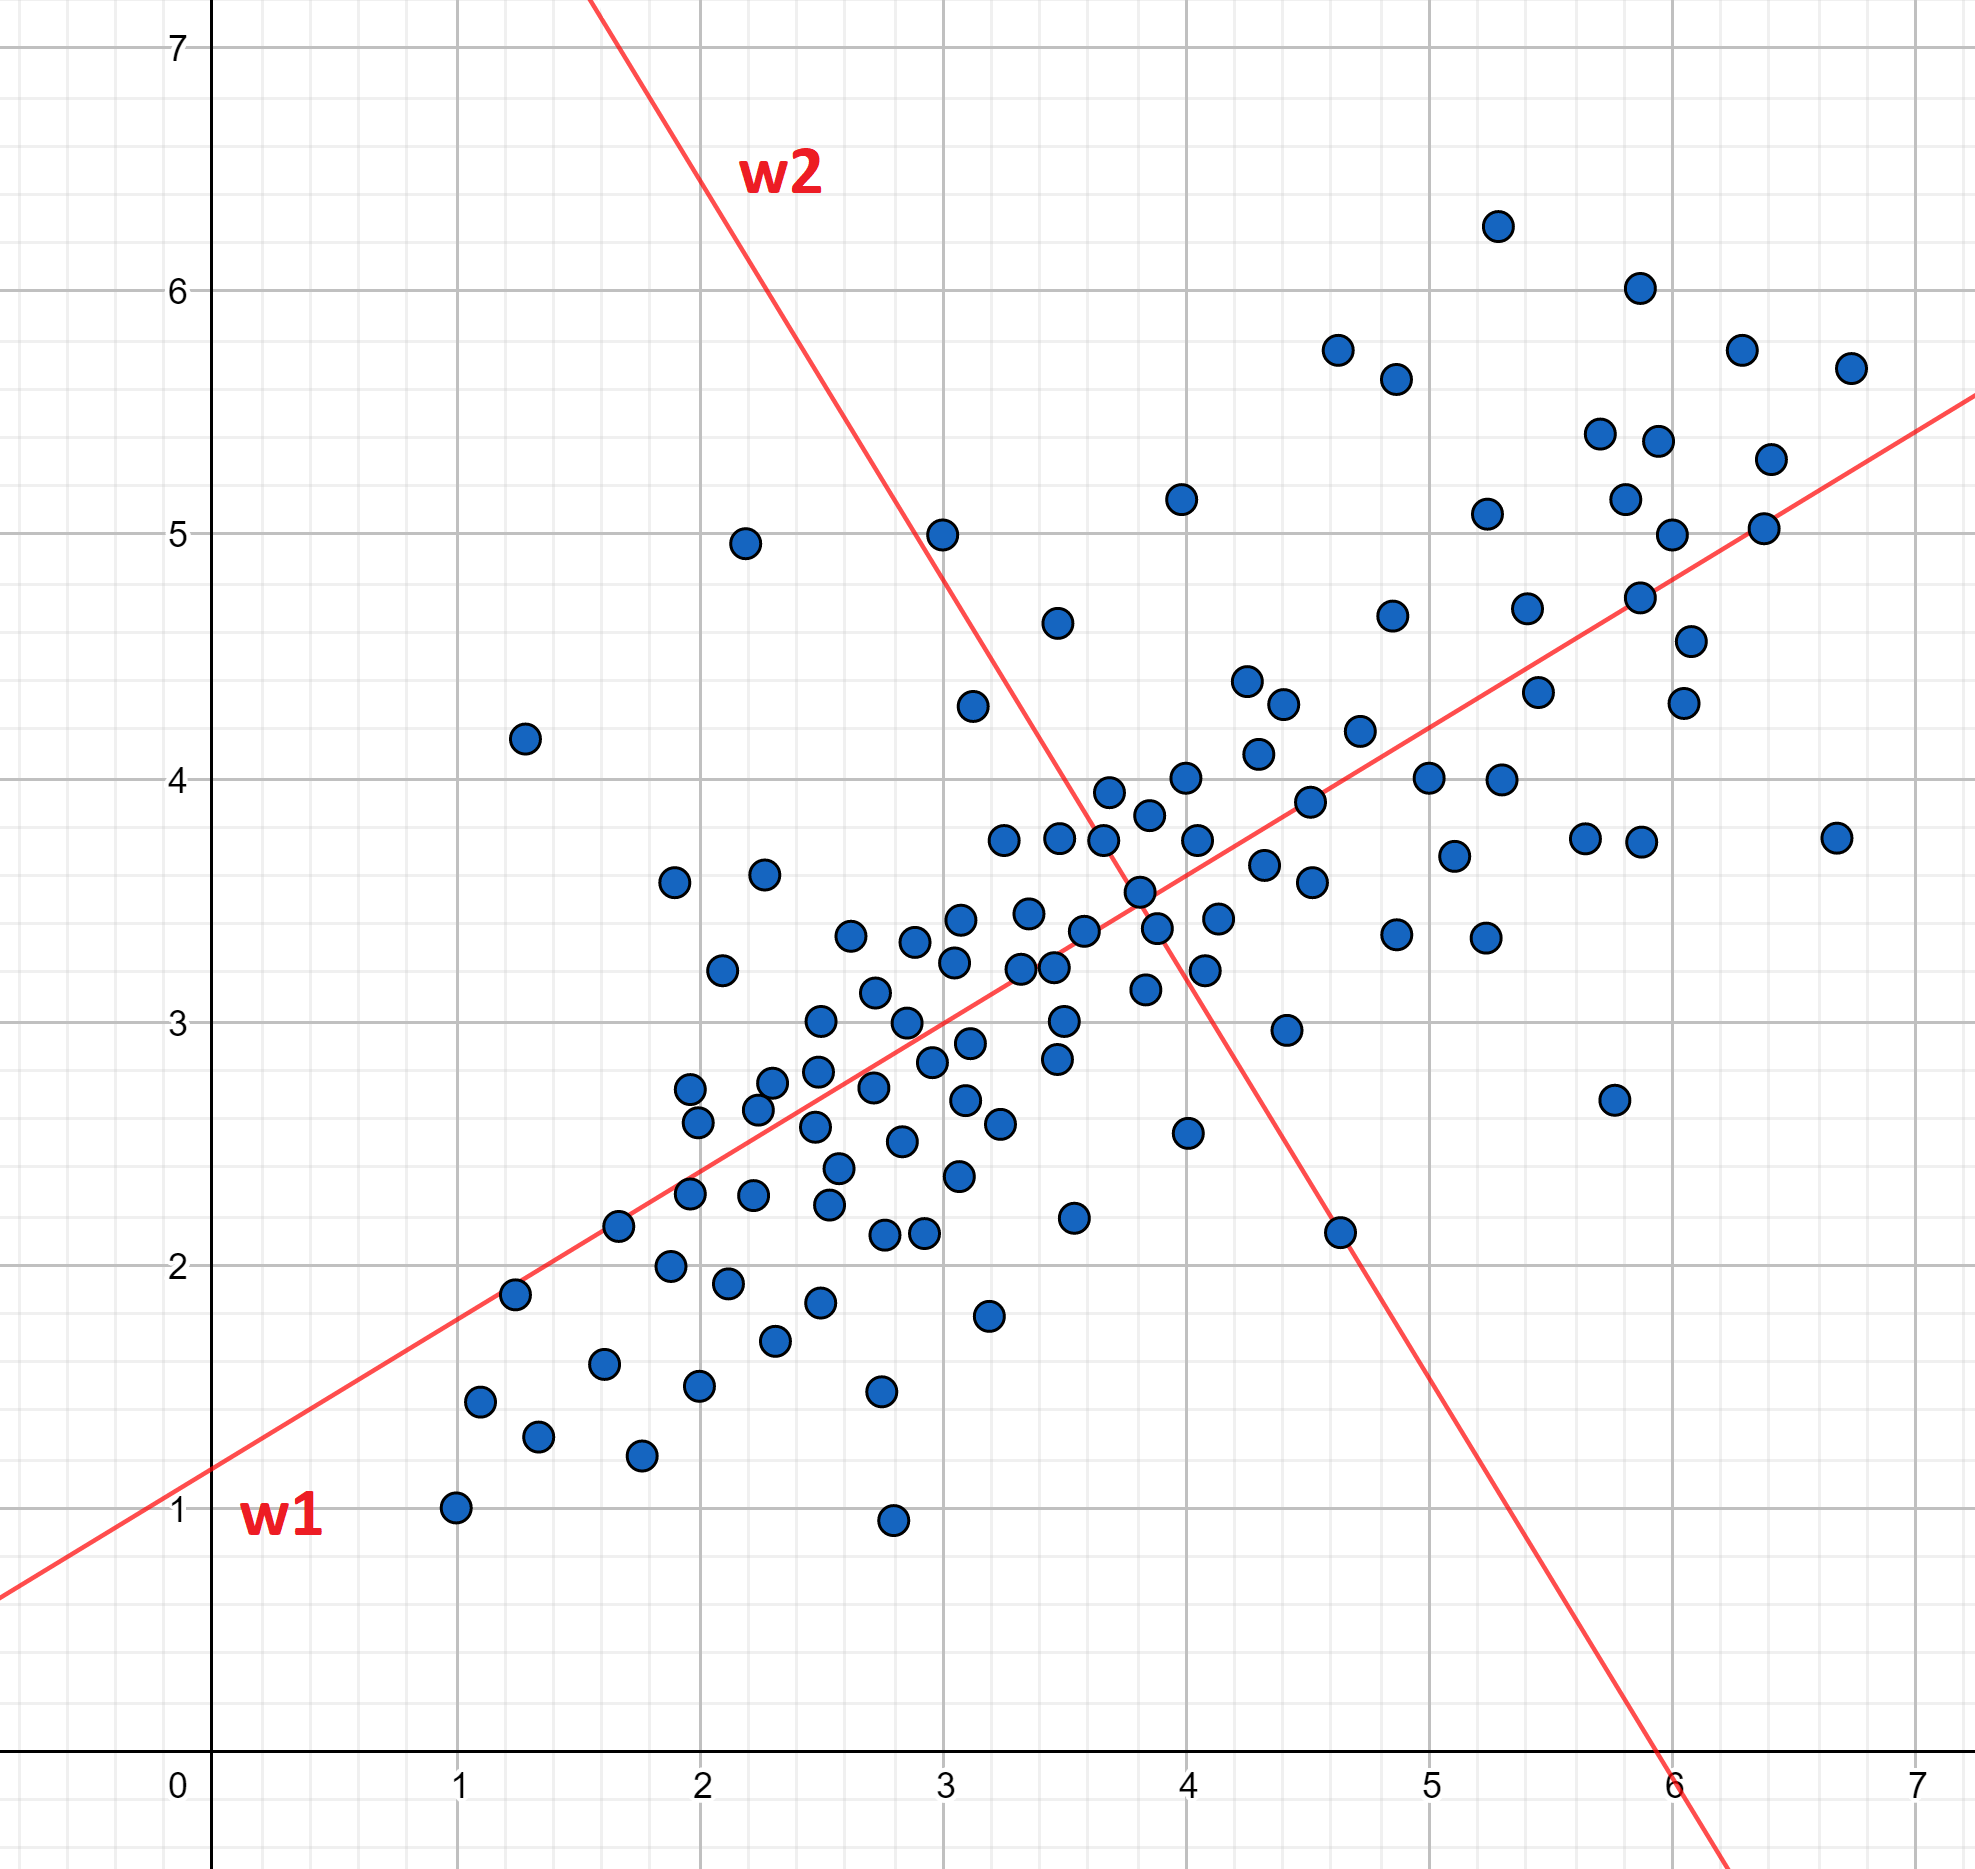
\includegraphics[width=0.4\textwidth]{tsc/pca_illustrated.png}
    \end{center}
    \caption{Illustration of how the principal components are found} 
    \label{fig:pca_illustrated}
\end{figure}

In ICA one assumes that the matrix of observed variables is a linear combination of mutually independent variables with an addition of noise, as illustrated in equation \ref{eq:ica_basics}. 
Where $X$ is the matrix of observed variables, $S$ is the matrix of independent hidden variables, $A$ is called a ''mixing matrix'' and $E$ is a noise matrix.  

\begin{equation}
    X = A S + E
    \label{eq:ica_basics}
\end{equation}

In ICA one aims to reconstruct $S$ as well as possible.
ICA is based on the central limit theorem which states that a sum of random variables with arbitrary probability distributions will tend towards a Gaussian distribution. 
Hence, one chooses $W$ such that the resulting independent components are mutually independent and show as little Gaussian properties as possible.

\section{Representation Methods} \label{sec:rep_methods}
There are numerous ways which a time series can be represented. 
\textcite{tsc_rev} define a time series representation given time series data $\{x_t\} = \{x_1, x_2, ... ,x_T\}$ as transforming the time series into another vector $\{x_t\} = \{\hat{x}_1, \hat{x}_2, ... ,\hat{x}_L\}$ where $L < T$. 
In theory $L=T$, but most often the point in transforming a time series is to reduce the amount of information present in the raw time series to more easily reveal patterns of interest. \bigskip

\begin{table*}[h]
    \centering
    \ra{1.3}
    \begin{tabular}{p{0.45\textwidth}p{0.3\textwidth}}
        \toprule
        Feature extraction method & Articles \\
        \midrule
        Basic signal statistics.                & \cite{ghsom_optimal_hedge_ratio, tsc_slaughterhouse, road_grade_china_pca_kmeans, auto_encoder_many_tsc_algorithms} \\
        PCA or ICA.                             & \cite{hysteresis_tsc_tensor_decomp, road_grade_china_pca_kmeans, load_tsc_state_space_model, multivariate_tsc_common_pca, ica_tsc_sea_level, copula_ica_tsc, tsc_slaughterhouse} \\
        % PCA                                   & \cite{hysteresis_tsc_tensor_decomp, road_grade_china_pca_kmeans, load_tsc_state_space_model, multivariate_tsc_common_pca, tsc_slaughterhouse} \\
        % ICA                                   & \cite{ica_tsc_sea_level, copula_ica_tsc} \\
        Time-frequency decomposition.           & \cite{shape_feat_mod_tsc_rfa, wavelet_multivar_tsc_multi_pca, ambient_air_vape_k_means, dwt_hac_kmeans_som, xml_dft_delaunay_traingulation, tsc_total_variation_distance, fragmented_periodogram, BSLEX_nonlin_nonstat_tsc}  \\
        Matrix, or tensor decomposition.        & \cite{multivar_tsc_riemann_manifold, fuzzy_c_means_pso_svd, svd_birch_tsc_stock_price, hysteresis_tsc_tensor_decomp, tensor_multi_elastic_kernel_tsc} \\
        % Covarience matrices.                  & \cite{multivar_tsc_riemann_manifold, } \\
        % Singular value decomposition (SVD).   & \cite{fuzzy_c_means_pso_svd, svd_birch_tsc_stock_price, } \\
        % Tensor decomposition.                 & \cite{hysteresis_tsc_tensor_decomp, tensor_multi_elastic_kernel_tsc} \\
        Symbolic aggregate approximation (SAX). & \cite{clust_large_datasets_aghabozorg, apxdist_sax_k_modes, shape_feat_mod_tsc_rfa} \\
        Permutation based coding.               & \cite{dependency_tsc_energy_markets} \\
        Spline functions.                       & \cite{hier_clust_w_state_space_models} \\
        Topological feature extraction.         & \cite{topology_for_shape_based_tsc} \\
        Autoencoder.                            & \cite{auto_encoder_many_tsc_algorithms} \\
        \bottomrule
    \end{tabular}
    \caption{Feature-based representation methods}
    \label{tab:feat_repr_meth}
\end{table*}

Table \ref{tab:feat_repr_meth} summarizes the different feature-based representation methods encountered in literature. 
%% Signal statistics 
Here the basic signal statistics category refers to the same values as in table \ref{tab:feat_ext_wt}: window average, max/min values and RMS values.
basic signal statistics are usually coupled with a form of dimensionality reduction such as PCA. 
%% ICA and PCA
\textcite{tsc_slaughterhouse, road_grade_china_pca_kmeans} both extract signal statistics from the time series they analyse (road grade time series \cite{road_grade_china_pca_kmeans}, and slaughterhouse health time series \cite{tsc_slaughterhouse}),
and then use PCA for dimensionality reduction. They then use euclidean distance to calculate the dissimilarity matrix between the time series.
\textcite{hysteresis_tsc_tensor_decomp} uses multivariate time series generated by a piezoelectric sensor-actuator system, 
then represent the time series with a 3-order hysteresis tensors.
They then use multilinear PCA to reduce the dimensionality of the tensor, and use a selv-developed tensor distance metric to measure similarity between the tensor representations.
\textcite{multivariate_tsc_common_pca} uses common PCA to represent the centers of clusters.
The principal components of the principal components are used to reconstruct the time series, and the reconstruction error is used as a similarity metric.
%% time frequency decomp
The category of time-frequency decomposition encompasses papers using the DWT, the continous wavelet transform, the DFT, spectral densities and fragmented periodograms.
\textcite{shape_feat_mod_tsc_rfa, ambient_air_vape_k_means, dwt_hac_kmeans_som} all use the DWT to decompose the time series signals. 
\textcite{shape_feat_mod_tsc_rfa} explores DWT as an alternative to other representation methods, while \textcite{ambient_air_vape_k_means, dwt_hac_kmeans_som} use DWT alone.
\textcite{fragmented_periodogram, BSLEX_nonlin_nonstat_tsc} both use periodograms to represent the time series to conserve some of the time-domain information about the signal. 
%% Matrix or tensor decomposition
\textcite{multivar_tsc_riemann_manifold} suggest representing multivariate time series with their covariance matrices, then projecting them to a tangent space and using the euclidean distance to measure the similarity between them.
\textcite{fuzzy_c_means_pso_svd, svd_birch_tsc_stock_price} both use singular value decomposition (SVD) to decompose multivariate time series. 
\textcite{fuzzy_c_means_pso_svd} uses SVD to represent the time series, and uses a particle swarm optimization to estimate the coefficients of an SVD representation of the cluster centre.
On the other hand, \textcite{svd_birch_tsc_stock_price} extract windows of the different time series, represent them using SVD, and then reconstruct them with a lower resolution.
Thus compressing the length time series, this approach can be considered a form of piecewise aggregate approximation. 
%% SAX and permutation based coding
SAX is also a form of piecewise aggregate approximation, but in SAX one represents segments of time series of specified length, with symbols.
This method is also used to compress the length of the time series. 
\textcite{clust_large_datasets_aghabozorg, apxdist_sax_k_modes} have an approach that uses SAX as a representation method for the time series, and both use the approximate distance as the similarity metric.
\textcite{shape_feat_mod_tsc_rfa} experiments with SAX as an alternative to the other approaches (AR model, and DWT). For the SAX representation they use the minimum distance between symbolic representations.
%% Permutation based
\textcite{dependency_tsc_energy_markets} suggest a system that extracts windows of the time series, and maps them to unique codewords based on how they permute.
They do this for all the univariate components of a multivariate time series object, 
and then use the frequency of occurence of different codeword combinations to construct a probability distribution of different codewords. 
Hence, they transform a multivariate time series into a probability distribution of codeword combinations. 
%% Topological
\textcite{topology_for_shape_based_tsc} analyze the trajectory of time series in phase-space. 
They then extract the topological features of the trajectory curves, such as the number of holes, birth time and death time of holes. 
Finally the measure similarity between time series as the euclidean distance between their topological features.
%% Autoencoder
\textcite{auto_encoder_many_tsc_algorithms} compare a feature-based representation method, to a raw-data based approach. 
In the feature-based approach they train an autoencoder to reconstruct the time series used, then they separate the autoencoder into the encoder and the decoder parts. 
They then used the compressed features at the output of the encoder as the representation of the time series in the clustering tasks. 
They then go on to test a multitude of different clustering algorithms to cluster the compressed features. \bigskip

\begin{table*}[h]
    \centering
    \ra{1.3}
    \begin{tabular}{p{0.45\textwidth}p{0.3\textwidth}}
        \toprule
        Time series model & Articles \\
        \midrule
        ARMA model.                 & \cite{garch_robust_tsc, shape_feat_mod_tsc_rfa, temporal_tsc_threshold_ar_models, tsc_ar_metric_air_pollution, ar_metric_trimmed_fuzzy_tsc_pm10, moar_mpl_tsc, struct_damage_ar_fuzzy_c_means, fstar_hac_tsc, var_multivar_tsc} \\  
        HMM.                        & \cite{mixture_gaussian_hmm, hmm_pm10_quantifying_impacts, multivariate_tsc_hmm} \\
        State space model.          & \cite{stock_price_tsc_regr_trees_som, load_tsc_state_space_model, hier_clust_w_state_space_models} \\
        Varience ratio statistics.  & \cite{financial_tsc_variance_ratio} \\
        Copula based model.         & \cite{copula_fuzzy_tsc_spatial} \\
        Network model.              & \cite{community_detection_networks_tsc, multivar_tsc_community_detection} \\
        \bottomrule
    \end{tabular}
    \caption{Model based representation methods}
    \label{tab:model_repr_meth}
\end{table*}

%% ARMA Model
Table \ref{tab:model_repr_meth} shows the different model based representation methods encountered, 
as one can see the ARMA model is the representation method most frequently encountered. 
However, within this approach there is also great variety, especially with regard to model complexity.
\textcite{shape_feat_mod_tsc_rfa, struct_damage_ar_fuzzy_c_means, ar_metric_trimmed_fuzzy_tsc_pm10, tsc_ar_metric_air_pollution} fit the time series with an AR model, and use the similarity between the AR-coefficients to cluster the time series. 
\textcite{garch_robust_tsc} models the time series with a generalized AR conditional heteroscedasticity model, which is a variation of the ARMA model that is better suited for non-stationary time series. 
More specifically, in GARCH models one models the variance of the innovations component as an ARMA model itself. 
They then test different similarity metrics based on squared Euclidean distance between the model coefficients to cluster the time series. 
\textcite{temporal_tsc_threshold_ar_models, fstar_hac_tsc} both use forms of threshold AR models. 
Threshold AR models aim to describe non-linear time series by splitting the time series into operational regimes using a threshold variable, and then modeling the different regimes with different linear AR models \cite{temporal_tsc_threshold_ar_models}. \textcite{temporal_tsc_threshold_ar_models} then tests 22 different distance metrics to measure similarity between the model coefficients, which is then used to cluster the time series. \textcite{fstar_hac_tsc} on the other hand, use the Wald statistic to test whether to time series are from the same generative process, and use the p-value as a distance measure.
\textcite{moar_mpl_tsc} use AR models to represent different clusters, and cluster the different time series as to which AR model is the most likely generative process for a given time series, using the expectation-maximization algorithm.
%% HMM
\textcite{mixture_gaussian_hmm} have a very similar approach to \textcite{moar_mpl_tsc}, just that they use HMMs to represent the clusters, and cluster the time series with regard to which HMM is the most likely generative process. 
\textcite{hmm_pm10_quantifying_impacts} represent air pollution time series with a HMM. 
The states of the HMM correspond to different long-term states of pollution emission levels.
They cluster the different time series based on which ''polution emission state'' each time series is in at a particular time. 
\textcite{multivariate_tsc_hmm} model each time series with a HMM, and then calculate the Kullback-Liebler distance between the likelihood of different observation sequences given the state and specific HMM. 
%% State space
\textcite{load_tsc_state_space_model} represents user electricity-load time series with a state space model. Individual time series are treated as dynamical systems with states in phase space. 
The states are then represented with mapping functions, and uses the euclidean distance between parameters of the mapping functions to cluster time series.
The state space representation of the time series is compared to a feature-based approach using PCA to compress signal statistics that are extracted from the electricity-load time series.
\textcite{stock_price_tsc_regr_trees_som} also explore the use of state space models, but to extract features of a time series.
% Spline
\textcite{hier_clust_w_state_space_models} compare a feature-based approach and a model-based approach for clustering time series. 
In the functional approach they represented as a linear combination of spline functions. 
The Euclidean distance between the vector of function coefficients associated with each time series is then used to measure similarity.
The idea behind their state space model approach is to model every observed time series as a linear combination of a set of hidden ''state'' time series. 
%% Varience rato and Copula
\textcite{financial_tsc_variance_ratio} use variance ratio statistics to represent the equity index time series, then they use cluster the time series into groups maximizing interdependence between the time series in clusters, and minimizing the interdependence between time series in different clusters. 
\textcite{copula_fuzzy_tsc_spatial} uses spatial multivariate time series. 
It extracts the spatial information from the multivariate time series, then goes on to decompose the univariate components into their deterministic and random components described in section \ref{sec:ts_models}.
The extracted innovation components are then represented by multivariate cumulative distribution functions, which are called copulas. 
The similarity metric for the multivariate time series is calculated as the $p$-norm of the difference between their copula representations.
%% Network model.
\textcite{community_detection_networks_tsc, multivar_tsc_community_detection} have a unique approach to clustering time series. 
\textcite{community_detection_networks_tsc} test a variety of similarity metrics to calculate the dissimilarity matrix between a set of univariate time series. 
They then use points to represent the time series, and use the measures of similarity to create vertices between the points to create a network model. 
To cluster the time series they then use community detection algorithms on the network model constructed. 
\textcite{multivar_tsc_community_detection} extends the model developed by \textcite{community_detection_networks_tsc} to be able to apply it to multivariate time series.
\textcite{multivar_tsc_community_detection} also develop an an algorithm based on non-negative matrix factorization to detect communities in the multivariate network model they use to represent the time series.

% \newpage
% \section{Similarity Metrics}
% One similarity metric is Euclidean distance.
% Another similarity metric is dynamic time warping.

% \begin{table*}[h]
%     \centering
%     \ra{1.3}
%     \begin{tabular}{p{0.45\textwidth}p{0.3\textwidth}}
%         \toprule
%         Similarity Metric & Articles \\
%         \midrule
%         Euclidean distance based metrics.   & \cite{financial_tsc_variance_ratio, hier_clust_w_state_space_models, topology_for_shape_based_tsc, community_detection_networks_tsc, shape_feat_mod_tsc_rfa, multivar_tsc_riemann_manifold, temporal_tsc_threshold_ar_models, ar_metric_trimmed_fuzzy_tsc_pm10, copula_ica_tsc, tsc_slaughterhouse, ambient_air_vape_k_means, dwt_hac_kmeans_som, xml_dft_delaunay_traingulation, svd_birch_tsc_stock_price, road_grade_china_pca_kmeans, fragmented_periodogram, auto_encoder_many_tsc_algorithms, load_tsc_state_space_model, struct_damage_ar_fuzzy_c_means, var_multivar_tsc, garch_robust_tsc, tsc_ar_metric_air_pollution, load_tsc_state_space_model,} \\
%         % Squared Euclidean distance.       & \cite{garch_robust_tsc, } \\
%         % Exponential Euclidean distance.   & \cite{tsc_ar_metric_air_pollution, load_tsc_state_space_model, } \\
%         Other $p$-norms.                    & \cite{community_detection_networks_tsc, copula_fuzzy_tsc_spatial} \\
%         Minkowski distance.                 & \cite{shape_feat_mod_tsc_rfa,} \\
%         Tensor distance metric.             & \cite{hysteresis_tsc_tensor_decomp, } \\
%         Matrix $L^p$ norms                  & \cite{tensor_multi_elastic_kernel_tsc} \\
%         Dynamic time warping distance (DTW).& \cite{community_detection_networks_tsc, shape_feat_mod_tsc_rfa, temporal_tsc_threshold_ar_models} \\
%         Approximate distance (APXDIST).     & \cite{clust_large_datasets_aghabozorg, apxdist_sax_k_modes} \\
%         MINDIST.                            & \cite{shape_feat_mod_tsc_rfa, } \\
%         Haussdorf distance.                 & \cite{temporal_tsc_threshold_ar_models, } \\
%         Aggregated quasi-distance.          & \cite{BSLEX_nonlin_nonstat_tsc, } \\
%         Kullback-Leibler distance.          & \cite{multivariate_tsc_hmm, } \\
%         Total variation distance.           & \cite{tsc_total_variation_distance, } \\
%         PCA similarity metric.              & \cite{wavelet_multivar_tsc_multi_pca} \\
%         Information based metrics.          & \cite{dependency_tsc_energy_markets, } \\
%         Pearson correlation coefficient.    & \cite{community_detection_networks_tsc, shape_feat_mod_tsc_rfa, fuzzy_c_means_pso_svd, } \\
%         Test statistic.                     & \cite{fstar_hac_tsc} \\
%         Principal component $R_e$.          & \cite{multivariate_tsc_common_pca} \\
%         \bottomrule
%     \end{tabular}
%     \caption{}
%     \label{tab:}
% \end{table*}

\section{Theory Behind Clustering Algorithms}
As mentioned before clustering is a form of unsupervised machine learning. 
The goal is to divide the dataset into clusters, by maximizing some similarity metric for members of the same cluster, 
and minimizing the same metric for members of different clusters.
In this section a detailed description will be given of the most common clustering algorithms enountered in literature.

\subsection{K-means family}
''K-means family'' is a collective term for a family of hard clusterimg algorithms where K-means is probably the most famous algorithm.
They all require the number of clusters ($K$) that the data should be divided into to be specified beforehand.
What differs between the algorithms in the K-means family is their representation of cluster centers.
The K-means algorithm represents the cluster centers with the mean of the members in the clusters, which is fairly intuitive.
The K-medoids algorithm represents the cluster centers with the medoid of the members in the clusters.
K-medoids is also called ''partitioning around medoids''.
The medoid in this context is the member of a cluster which has the smallest average dissimilarity to the other members of the cluster. 
The advantage of K-medoids, over K-means is that it represents the cluster centers with actual members of the clusters, instead of a virtual average. 
This can be computationally efficient when dealing with data objects of large size, such as time series. \bigskip

The general family of K-means algorithms work iteratively. In the first iteration the cluster centers are randomly initialized, 
then the dissimilarity between all data objects and the cluster centers are calculated, 
the data objects are then assigned to the cluster with the minimal dissimilarity to the cluster center,
the cluster centers are updated and algorithm repeats by recalculating the dissimilarity between all points and the different cluster centers.
These steps are repeated untill the cluster centers, and membership assignments converge.
The biggest disadvantages with the family of K-means algorithms are that they can be stuck in local optimums, 
and that the number of clusters have to be specified beforehand.

\subsection{Fuzzy C-means family}
The fuzzy C-means family of algorithms are equal to the family of K-means algorithms in all ways except one. 
The family of C-means algorithms are said to be \textit{soft} clustering algorithms. 
This means that all data objects can have a degree of memberships to all clusters, where as in the family K-means algorithms data objects can only be members of one cluster.
This fuzziness property leads to two other parameters that must be defined.
The power of membership degree which decides how many clusters each data object can be members of, 
and the degree of membership matrix which keeps track of the membership degrees of all data objects.
The power of membership degree must be fixed together with the number of clusters, and the degree of membership matrix is updatated each iteration.

\subsection{Hierarchical clustering}
Hierarchical clustering algorithms come in many flavours, but they all build hierarchies of clusters \cite{espen}.
A great advantage with hierarchical clustering algorithms is that the number of clusters is not specified beforehand. 
Hierarchical clustering algorithms can be split into agglomorative, and divisive algorithms.
Agglomorative hierarchical clustering algorithms start with all data objects as their own clusters, then iteratively merges clusters together until there is only one cluster containing all data objects.
Divise hierarchical clustering starts with one cluster containing all data objects, and then iteratively splits the clusters into smaller clusters until every data object is contained in a separate cluster.
To decide which clusters should be merged during a given iteration, the algorithm uses the similarity between clusters, which is called the \textit{linkage criterion}.
There are four main types of linkage criteria: 
\begin{itemize}
    \item Single linkage:   Computes the similarity between two clusters as the dissimilarity as the dissimilarity between the two most similar data objects in each cluster \cite{dependency_tsc_energy_markets}.
    \item Complete linkage: Computes the similarity between two clusters as the dissimilarity as the dissimilarity between the two least similar data objects in each cluster \cite{financial_tsc_variance_ratio}.
    \item Average linkage:  Computes the similarity between two clusters as the average dissimilarity between all points in each cluster \cite{dependency_tsc_energy_markets}.
    \item Wards linkage:    Computes the similarity between two clusters as the increase in sum of squared error by merging the two clusters \cite{copula_ica_tsc}.
\end{itemize}

After the algorithm has created a hierarchy of clusters, it produces what is called a dendrogram which shows what the different clusters would look like for a different number of clusters. 
The correct structure is then found by cutting the dendrogram at the appropriate number of clusters. 
The appropriate cutting of the dendrogram is chosen by calculating indices that evaluate the inter- and intra cluster variance such as the silhuette index \cite{BSLEX_nonlin_nonstat_tsc, copula_ica_tsc}, Duda-Hart index \cite{financial_tsc_variance_ratio} and Dunn's index \cite{tsc_total_variation_distance}.
Another advantage of the hierarchical clustering algorithm is that it is deterministic in it's cluster hierarchy, 
meaning that it will always produce the same dendrogram if it is given the same dissimilarity matrix \cite{espen}.

\subsection{Expectation-maximization}

\subsection{Self-organizing maps}

\subsection{Spectral clustering}

\section{Clustering Algorithms}

\begin{table*}[h]
    \centering
    \ra{1.3}
    \begin{tabular}{p{0.45\textwidth}p{0.3\textwidth}}
        \toprule
        Clustering Algorithm & Articles \\
        \midrule
        K-means family 						                                & \cite{financial_tsc_variance_ratio, hier_clust_w_state_space_models, topology_for_shape_based_tsc, multivariate_tsc_hmm, apxdist_sax_k_modes, temporal_tsc_threshold_ar_models, ambient_air_vape_k_means, hysteresis_tsc_tensor_decomp, dwt_hac_kmeans_som, road_grade_china_pca_kmeans, auto_encoder_many_tsc_algorithms} \\
        Fuzzy C-means family 				                                & \cite{garch_robust_tsc, copula_fuzzy_tsc_spatial, temporal_tsc_threshold_ar_models, tsc_ar_metric_air_pollution, wavelet_multivar_tsc_multi_pca, ar_metric_trimmed_fuzzy_tsc_pm10, fuzzy_c_means_pso_svd, struct_damage_ar_fuzzy_c_means} \\
        Hierarchical clustering 			                                & \cite{financial_tsc_variance_ratio, hier_clust_w_state_space_models, BSLEX_nonlin_nonstat_tsc, shape_feat_mod_tsc_rfa, ica_tsc_sea_level, multivar_tsc_riemann_manifold, tsc_total_variation_distance, dependency_tsc_energy_markets, copula_ica_tsc, tsc_slaughterhouse, dwt_hac_kmeans_som, auto_encoder_many_tsc_algorithms, fstar_hac_tsc} \\
        Balanced Iterative Reducing and Clustering using Hierarchies (BIRCH)& \cite{svd_birch_tsc_stock_price, auto_encoder_many_tsc_algorithms} \\
        Self-organizing map (SOM) 			                                & \cite{ghsom_optimal_hedge_ratio, stock_price_tsc_regr_trees_som, dwt_hac_kmeans_som} \\
        Expectation-maximization 			                                & \cite{mixture_gaussian_hmm, moar_mpl_tsc, auto_encoder_many_tsc_algorithms, hier_clust_w_state_space_models} \\
        Spectral clustering 				                                & \cite{temporal_tsc_threshold_ar_models, fragmented_periodogram, auto_encoder_many_tsc_algorithms} \\
        % HMM                                                               & \cite{hmm_pm10_quantifying_impacts} \\ % hvis du først skal ha med state space kan du også ha med HMM
        % State space models                                                & \cite{hier_clust_w_state_space_models} \\
        % Community detection algorithms	                                & \cite{community_detection_networks_tsc, multivar_tsc_community_detection} \\
        % Matrix factorization 				                                & \cite{multivar_tsc_community_detection} \\
        % Delauney Triangulation method 	                                & \cite{xml_dft_delaunay_traingulation} \\
        Affinity propagation  				                                & \cite{auto_encoder_many_tsc_algorithms} \\
        DBSCAN  							                                & \cite{auto_encoder_many_tsc_algorithms} \\
        Mean shift  						                                & \cite{auto_encoder_many_tsc_algorithms} \\
        Custom algorithms 					                                & \cite{clust_large_datasets_aghabozorg, multivariate_tsc_common_pca, tensor_multi_elastic_kernel_tsc, var_multivar_tsc, xml_dft_delaunay_traingulation} \\
        \bottomrule
    \end{tabular}
    \caption{Clustering algorithms encountered in literature}
    \label{tab:clust_alg}
\end{table*}
Table \ref{tab:clust_alg} shows the different clustering algorithms encountered in the literature. 
%% K-means

%% K-medoids

%% K-median

%% K-modes

%% Fuzzy C-means

%% Fuzzy C-medoids

% Hierarchical clustering

%% BIRCH

%% SOM
Not relevant because hard to interpret.
%% EM
The expectation-maximization algorithm is used for clustering when each cluster center is represented by a mixture model. 
The mixture models used to represent the cluster centers that have been enountered in literature are: ARMA models \cite{moar_mpl_tsc}, HMM \cite{mixture_gaussian_hmm}, Gaussian distributions \cite{auto_encoder_many_tsc_algorithms} and state space models \cite{hier_clust_w_state_space_models}.
Common for all the articles is that they use expectation-maximization to assign the time series to the cluster which has the most likely generative process as cluster center.

% Affinity propagation, mean shift, DBSCAN
As mentiond in section \textcite{auto_encoder_many_tsc_algorithms} use the encoder part of an autoencoder to compress the time series produced by an energy research center. 
The test hierarchical clustering, K-means, spectral clustering, expectation-maximization, BIRCH, affinity propagation, mean shift and DBSCAN to cluster the compressed features. 
The feature-based approach is compared to a raw-data based approach, and they found that the feature-based had better accuracy on a labelled dataset.

\section{Discussion}
In this chapter different representation methods, and clustering algorithms encountered in the literature have been explored. 
Of the feature-representation methods PCA, and ICA are the most viable option for reducing the dimensionality of multivariate time series.
Because they build on strong theoretical ground, without being overly complex methods they are straight forward to apply, and should be considered as a representation method for the master thesis. 
PCA will in fact be tested for exploring the data from a particular wind farm in chapter \ref{chap:data_exp}.
The piecewise aggregate approximation techniques of SAX and permutation based coding are also quite clear and could be considered for application in the master thesis.
The other feature-based representation methods show great promise, but are not appropriate for the for exploration in the master thesis.
The use of an autoencoder for feature extraction explored by \textcite{auto_encoder_many_tsc_algorithms} showed great promise in terms of classification accuracy, compared to the raw-data approach.
However, it suffers the same issues as the regression based models described in section \ref{sec:reg_bas_mod}, a lack of interpretability. 
Of the model-based representation methods ARMA models were found to be a frequent model used, 
and the fact that there is such a great variation in the individual approaches means that there might be a flavour of ARMA models that could be used to model the time series produced by wind turbines.
Additionally, the use of ARMA models to model the time series produced by wind turbines, or wind turbine components has already been explored \cite{ml_cm_wt_blade_ARMA_2018, fault_detection_and_isolation_using_classifier_fusion, lin_and_non_lin_feat_for_ice_detection_on_blades, dirt_n_mud_detection_using_guided_waves, vibration_ARMA_decision_tree_cm_wt}, which strengthens the argument that they are a representation method that should be explored in the master thesis. % Kanskje ta denne setningen i den siste diskusjonen
The HMM is a model-based approach that has showed great promise in terms of representing time series, and has even be used to cluster the time series \cite{hmm_pm10_quantifying_impacts} in a simple manner.
The approach of \textcite{hmm_pm10_quantifying_impacts} of representing all time series with the same HMM, and then clustering together time series which are in the same state is simple, but also elegant.
It is elegant because it yields a simple method of observing how the different time series traverse through different clusters over time, which is quite usefull for long-term observation of a wind farm. 
The approaches that represent time series with different HMM models, and measure dissimilarity based on model parameters \cite{} should also be considered for the master thesis.


